\section{Experimental Methodology} \label{sec:c3_method}

% How you obtain the data?
% Add a figure of procedures.
% Source code

% Figure of setup/experiment if possible. asdf

The presented model (\eref{eq:texepercent}) was utilised to explore the sizing effect of energy storage. 
An existing IPS was implemented and profiled to configure the model. 
With the configured model, the relationship between forward progress and other system parameters was explored. 
The modelled results were then validated with the implemented IPS.
For reproducing and understanding the method and results, the source code of the model and the implemented IPS is available online\footnote{\url{https://git.soton.ac.uk/energy-driven/energy-storage-sizing}}.

\begin{figure}
    \centering
    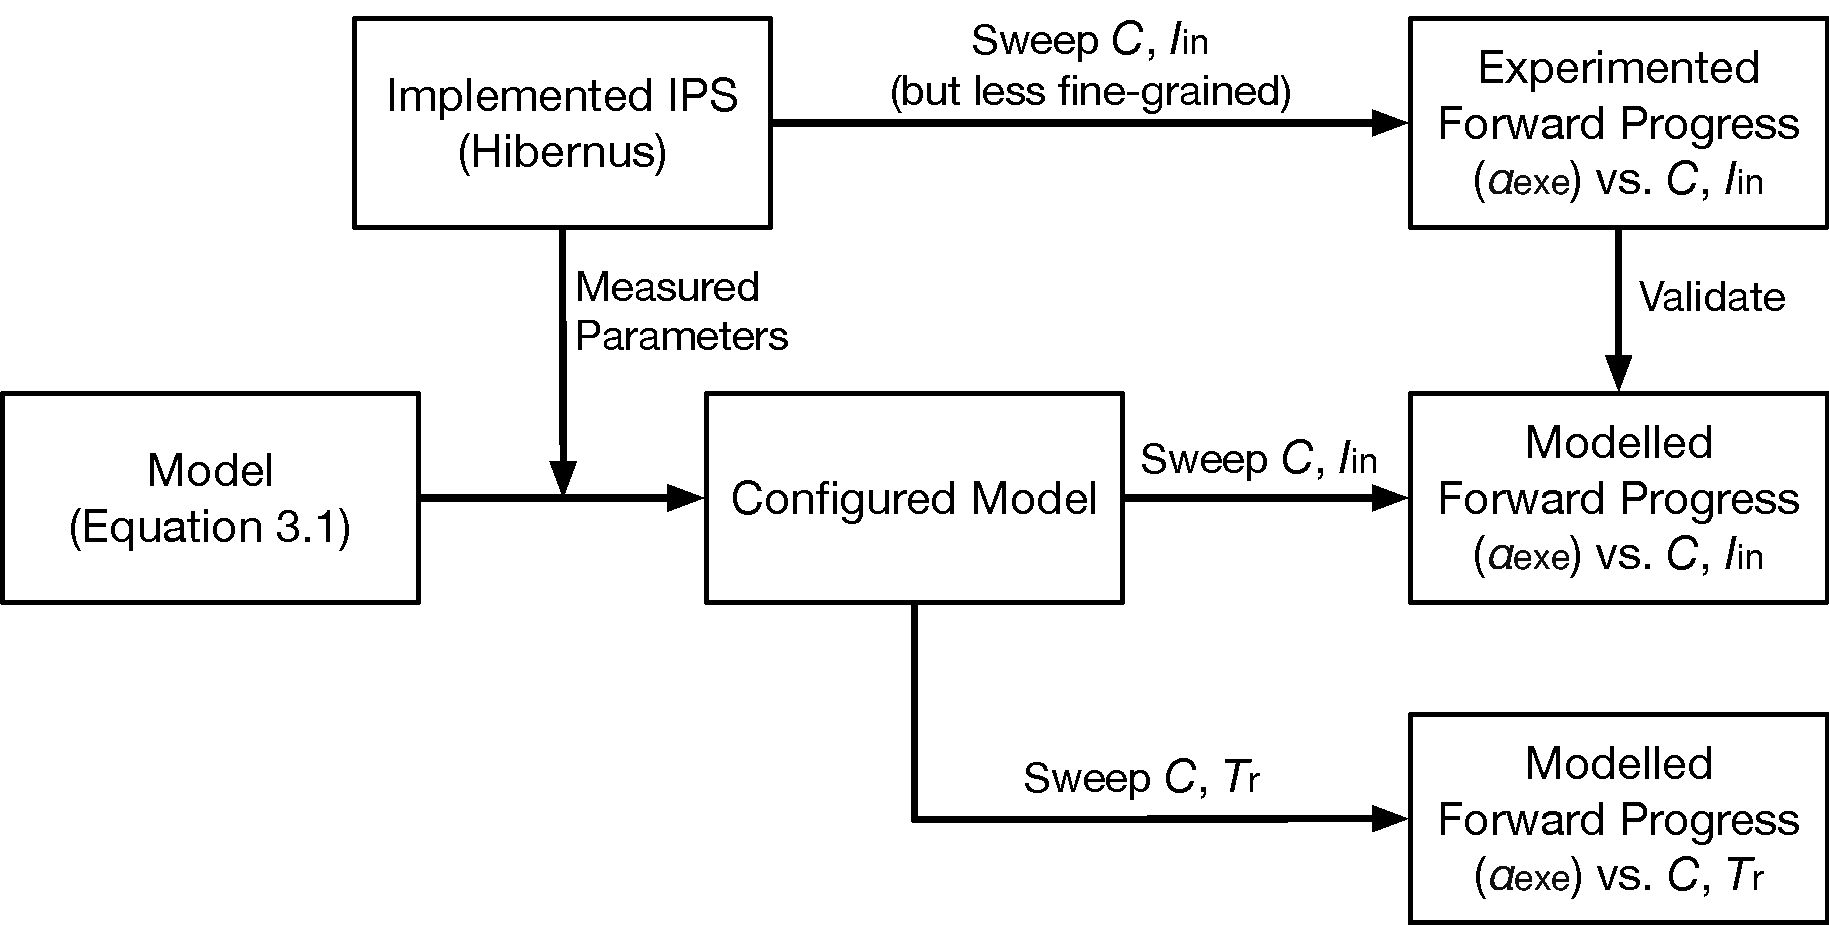
\includegraphics[width=\columnwidth]{ch3_sizingeffect/figures/procedure}
    \caption{Methodology of Model Exploration and Experimental Validation. }
    \label{fig:procedure} 
\end{figure}

The modelling and experimental methodology is shown in \fref{fig:procedure}.
The initial model (\eref{eq:texe}) estimates theoretical forward progress as presented in \sref{sec:c3_model}. 
The energy storage in the model was configured based on an empirical capacitor leakage model (with detail presented in \sref{ssubsec:estor_model}).
An IPS based on Hibernus~\cite{balsamo2015hibernus} was implemented and its load parameters were profiled so as to configure the load model (with detail presented in \sref{ssubsec:loadconfig}).
With the configured model, a range of the energy storage size (\N{C}, supply current (\nm{I}{in}), and volatile state size (equivalent to restore time \nm{T}{r} in Hibernus-like IPSs) were swept with a fine granularity and the corresponding forward progress was generated, so as to investigate their relationship against forward progress (\nm{T}{exe}).
Finally, the actual forward progress was measured on the implemented IPS with a smaller set of \N{C} and \nm{I}{in} for validation of modelled results. 

\subsection{Model Configuration}

The model was configured with an empirical capacitor model and experimentally measured load characteristics so as to approximate a real IPS platform. 

\subsubsection{Energy Storage} \label{ssubsec:estor_model}

The energy storage is represented as an ideal capacitor with empirically defined leakage current. 
Its terminal voltage is directly applied to the load, so is modelled as:
\begin{equation}
  C \frac{d\nmm{V}{cc}}{dt} = \nmm{I}{harv} - \nmm{I}{load} - \nmm{I}{leak}
\end{equation}
where \nm{I}{load} is the current consumption of the load. 
In this exploration, we refer to the empirical \nm{I}{leak} of AVX TAJ low-profile series tantalum capacitors~\cite{tancap1}, which depends on capacitance $C$, rated voltage \nm{V}{rated}, and terminal voltage \nm{V}{cc}~\cite{avxleakage}:
\begin{equation}
    % aluminium 
%   \nmm{I}{leak} = max\{0.03 C \nmm{V}{rated}, \quad 4 \times 10^{-6}\}    \quad (A)
    % tantalum
    \nmm{I}{leak} = 0.01 \lambda C \nmm{V}{rated} \quad (A)
\end{equation}
where $\lambda$ denotes the ratio of the actual current leakage at \nm{V}{cc} to the current leakage at \nm{V}{rated}, and $\lambda$ is approximated as: 
\begin{equation}
    \lambda = 0.05 \times 20^{\frac{\nmm{V}{cc}}{\nmm{V}{rated}}}
\end{equation}
We assume a typical load of $<$ \SI{4.0}{\volt} so, to minimise leakage, we select a device with $\nmm{V}{rated} =$ \SI{10}{\volt} so as to operate between 25-40\% of its rated voltage~\cite{avxleakage}. 

% Here, \nm{V}{cc} affects both the energy harvester and the load. On the harvester side, \nm{V}{cc} is the operating voltage of PV cells, which has an effect on the harvested current $I_{harvest}$. On the load side, \nm{V}{cc} is the supply voltage, which determines when the load wakes up or powers off (affecting \nm{I}{load}). Hence, the energy storage, the energy harvester, and the load impact on each other through \nm{V}{cc}, $I_{harvest}$, and \nm{I}{load}. 

\subsubsection{Intermittent Computing Load} \label{ssubsec:loadconfig}

We configured the load with experimentally measured current draws and time overheads.
We only consider computational loads in this study, as handling of peripherals in intermittent systems is still an ongoing research topic~\cite{rodriguez2018restop, Maeng:2019:SPI:3314221.3314613}. 

We implemented and parameterised a reactive IPS~\cite{balsamo2015hibernus} on a TI MSP430FR6989-based development board. 
The load parameters were profiled with the MCU running a Dijkstra path finding algorithm with \SI{1696}{\byte} RAM usage at \SI{8}{\mega\hertz}. 
The supply voltage monitoring circuits use the MCU's internal comparator and an external \SI{3}{\mega\ohm} voltage divider. 
The restore and save voltage thresholds are set as \nm{V}{r} = \SI{2.4}{\volt} and \nm{V}{s} = \SI{2.1}{\volt} respectively. 
The MCU shutdown voltage \nm{V}{off} is \SI{1.8}{\volt}. 

The measured current draws and time overheads are listed in \tref{tab:load}.
The current draw was profiled with experimental measurements at a range of supply voltages. 
The variation of \nm{I}{lpm} between \nm{V}{off} (\SI{1.8}{\volt}) and \nm{V}{r} (\SI{2.4}{\volt}) is 2\%, and for \nm{I}{exe} between \nm{V}{s} (\SI{2.1}{\volt}) and \SI{3.3}{\volt} is 1.5\%. 
\nm{I}{exe} also has a run-time variation of 2.8\% due to a variable memory access rate. 
As these variations of \nm{I}{exe} and \nm{I}{lpm} in their effecting voltage range are minor, we therefore omit the variations and use the mean of \nm{I}{exe} and \nm{I}{lpm} in the model. 
\nm{I}{r} and \nm{I}{s} are measured at \nm{V}{r} and \nm{V}{s} respectively. 

Given the voltage thresholds and the current consumption, the minimum energy storage capacitance is \SI{6.2}{\micro\farad}. 
This guarantees that a save and restore operation can complete even if the incoming supply current drops instantaneously to zero. 
Moreover, the model parameters in \tref{tab:load} are given as an example, and can be changed for different load characteristics. 
For example, \nm{T}{r} and \nm{T}{s} can be tuned for different volatile state sizes.

\begin{table}
    \renewcommand{\arraystretch}{1.2}
    \centering
    \begin{tabular}{|c|c|}
    \hline
    \textbf{Parameter} & \textbf{Value}\\
    \hline
    \nm{I}{exe} & \SI{887}{\micro\ampere}\\
    \nm{I}{lpm} & \SI{26}{\micro\ampere}\\
    \nm{I}{r} & \SI{971}{\micro\ampere}\\
    \nm{I}{s} & \SI{811}{\micro\ampere}\\
    \nm{T}{r} & \SI{1.903}{\milli\second}\\
    \nm{T}{s} & \SI{1.880}{\milli\second}\\
    % \multicolumn{2}{c}{Measured Parameters}\\
    % \hline
    % $I_{exe}, I_{R}, I_{S}$ & 0.87 mA\\
    % \nm{I}{lpm} & 0.40 mA\\
    % \nm{T}{r} & 2.298 ms\\
    % \nm{T}{s} & 2.274 ms\\
    % \hline
    % \multicolumn{2}{c}{Simulation Parameters}\\
    % \hline
    % $I_{exe}, I_{R}, I_{S}$ & 1.00 mA\\
    % \nm{I}{lpm} & 0.01 mA\\
    \hline
    \end{tabular}
    \caption{Profiled MCU parameters.}
    \label{tab:load}
\end{table}
